\section{系统架构与关键技术}
\label{sec:method}

\subsection{分层系统架构与关键技术}

FP-FraudSim采用离线训练与在线推理协同的五层架构。数据与仿真层负责多源融合、七类诈骗注入和可调交易仿真；流式计算层负责Kafka事件解耦、Flink事件时间、watermark和滑动窗口；特征与智能层负责Redis画像、多维特征、LightGBM主模型及图挖掘旁路；决策与应用层负责风险分级、理由码、团伙溯源和可视化；反馈与治理层负责人工反馈、候选评估、受控发布、回滚、审计与安全。分层架构如图~\ref{fig:fraudsim_architecture}所示。

\begin{figure}[H]
  \centering
  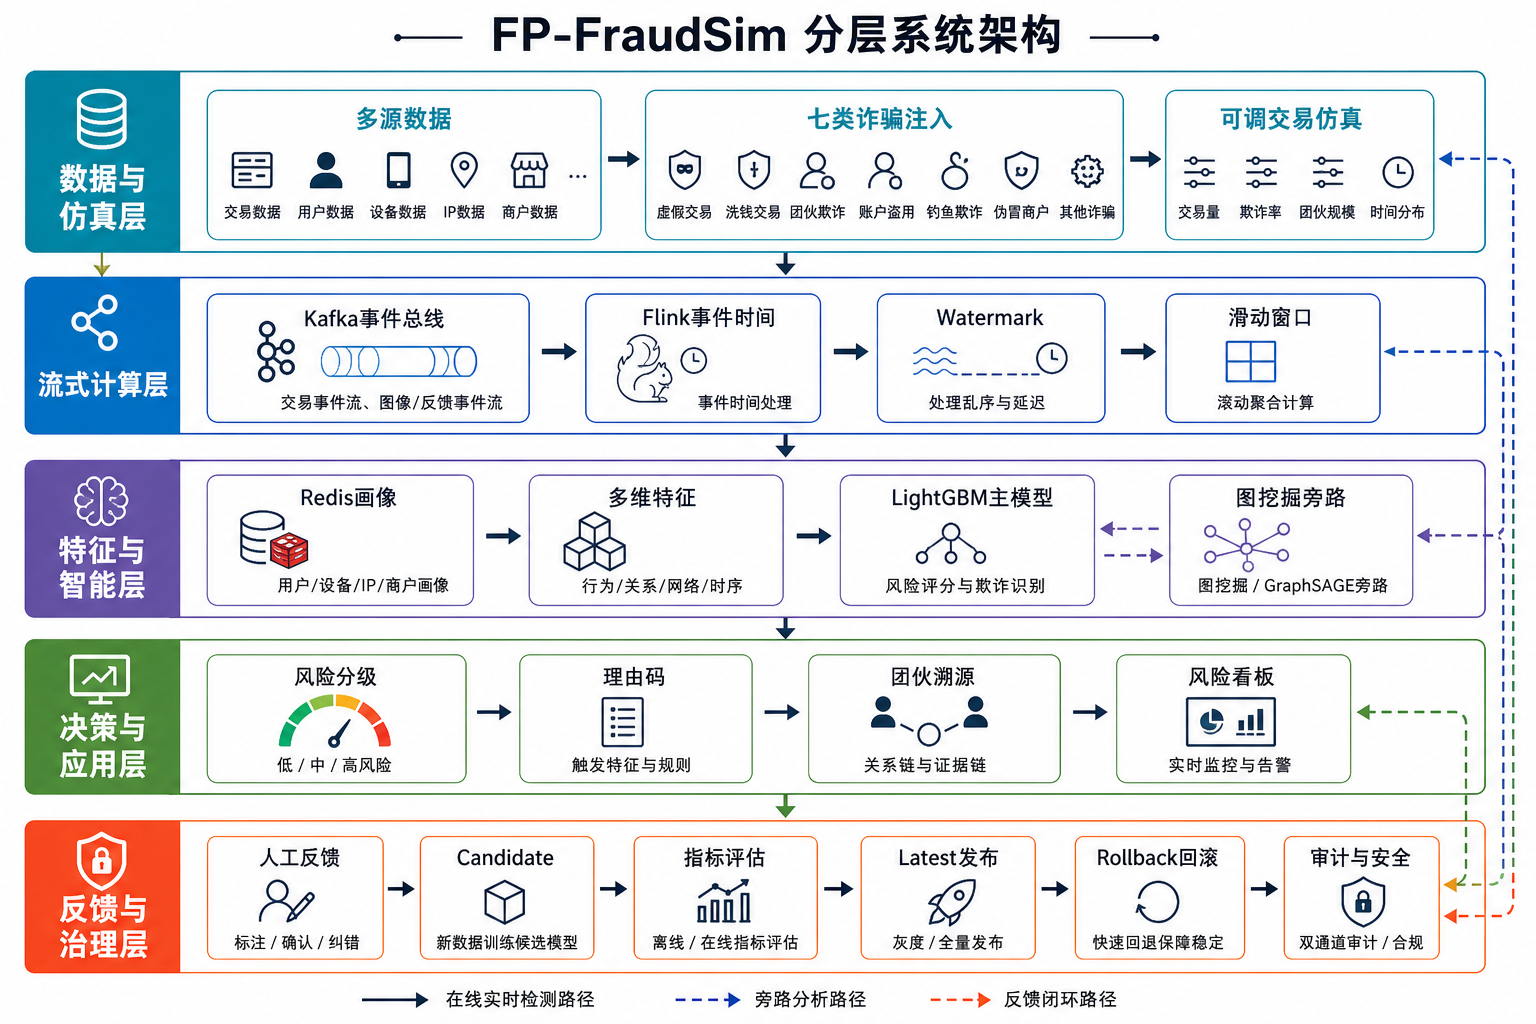
\includegraphics[width=\textwidth]{pic/layered_system_architecture_image2.png}
  \caption{FP-FraudSim分层系统架构与闭环路径}
  \label{fig:fraudsim_architecture}
\end{figure}

部署上使用Docker Compose编排Kafka、Redis、Model API、Flink JobManager、Flink TaskManager和Flink风险作业，完成单机最小闭环验证。项目进一步提供\code{deploy/k8s/edge.yaml}和\code{center.yaml}：边缘/私有云实时侧部署Kafka、Redis、双副本Model API、Flink和NetworkPolicy；中心云训练侧以CronJob运行反馈候选训练和GraphSAGE旁路实验。清单包含PVC、Secret和资源约束，为后续接入对象存储、镜像仓库和跨云加密同步提供基础。

\subsubsection{框架选型与流式框架}

系统架构围绕实时反诈业务约束进行选型，而非简单堆叠组件。Kafka承担高吞吐事件总线，将交易生产、风险计算、告警和反馈解耦；即使模型服务短时波动，交易事件仍可在消息队列中保留并重放。Flink提供有状态计算、事件时间、watermark和checkpoint机制，能够在乱序交易流中稳定维护短时行为窗口，这是普通HTTP同步调用或定时批处理难以完整实现的能力。Redis以键值方式保存用户、设备、IP、商户和图画像，使在线链路无需重复扫描历史数据即可完成毫秒级画像补齐。FastAPI将模型推理独立为服务，使模型训练、流计算和推理资源能够分别扩缩容，并通过统一接口支持模型热切换。

该组合兼顾了\textbf{吞吐、延迟、容错、扩展与迭代}：Kafka和Flink适合交易流水平扩展；checkpoint和结果主题支持故障恢复与审计；Redis降低在线特征读取成本；模型服务与流计算解耦，使算法升级不需要重写实时链路。系统同时提供同步单笔和微批评分模式，能够根据业务流量在即时响应与吞吐效率之间动态取舍。

\subsection{业务逻辑流程设计}

交易流从\code{transaction\_events}主题进入Flink。在线评分作业\code{fraudsim/streaming/flink\_job.py}实现两种评分模式：同步单笔评分和微批评分。微批模式根据批大小和等待时间聚合记录，默认批大小为50、等待时间为300毫秒，再调用FastAPI批量\code{/predict}接口，以降低HTTP调用开销。

Flink作业对每条交易执行以下步骤：

\begin{enumerate}
  \item 解析JSON事件并提取事件时间；
  \item 维护用户、设备、IP、商户四类内存滑动窗口；
  \item 计算5分钟、10分钟和1小时窗口特征；
  \item 从Redis读取用户、设备、IP、商户和图画像；
  \item 调用模型服务输出风险分数、等级、处置动作和理由码；
  \item 将完整结果写入\code{risk\_results}，将高风险结果写入\code{alert\_events}，将迟到事件写入\code{late\_events}。
\end{enumerate}

该设计满足赛题关于“交易发生的同时完成风险评估与欺诈判定”的要求，同时保留结果主题便于回放、审计和答辩展示。

图~\ref{fig:realtime_decision_flow}进一步展示了单笔交易从进入流式链路到形成业务处置的过程。模型分数不是最终结果，系统还需要结合阈值、理由码和图证据生成可执行决策。

\begin{figure}[H]
  \centering
  \resizebox{\textwidth}{!}{%
  \begin{tikzpicture}[node distance=0.62cm and 0.55cm]
    \node[flowcard=flowcyan] (event) {\textcolor{white}{\bfseries 交易事件}\nodepart{second}Kafka输入};
    \node[flowcard=flowblue, right=of event] (feature) {\textcolor{white}{\bfseries Flink实时特征}\nodepart{second}窗口统计\\画像补齐};
    \node[flowcard=flowpurple, right=of feature] (score) {\textcolor{white}{\bfseries 模型服务}\nodepart{second}风险分数\\理由码};
    \node[decisioncard, right=0.7cm of score] (decision) {两级阈值判断};
    \node[flowcard=flowgreen, above right=0.55cm and 0.8cm of decision] (pass) {\textcolor{white}{\bfseries 低风险}\nodepart{second}直接放行};
    \node[flowcard=floworange, right=0.8cm of decision] (review) {\textcolor{white}{\bfseries 中风险}\nodepart{second}人工复核};
    \node[flowcard=flowred, below right=0.55cm and 0.8cm of decision] (reject) {\textcolor{white}{\bfseries 高风险}\nodepart{second}拒绝并告警};
    \draw[flowarrow] (event) -- (feature);
    \draw[flowarrow] (feature) -- (score);
    \draw[flowarrow] (score) -- (decision);
    \draw[flowarrow] (decision) -- node[flowlabel, above, sloped]{低于审核阈值} (pass);
    \draw[flowarrow] (decision) -- node[flowlabel, above]{介于两阈值} (review);
    \draw[flowarrow] (decision) -- node[flowlabel, below, sloped]{高于拦截阈值} (reject);
  \end{tikzpicture}
  }
  \caption{实时风险评分与分级处置流程}
  \label{fig:realtime_decision_flow}
\end{figure}

\subsection{数据结构设计与组织}

系统以交易事实表为中心，通过画像表、图结构和事件主题组织数据。离线Parquet保证大规模分析与可复现训练效率，在线JSON事件保证Kafka传输兼容性，Redis键值画像保证低延迟查询，图节点与图边保证团伙关系可追溯。核心结构如表~\ref{tab:data_structure_design}所示。

\begin{table}[H]
  \centering
  \caption{核心数据结构与组织方式}
  \label{tab:data_structure_design}
  \renewcommand\arraystretch{1.32}
  \setlength{\tabcolsep}{4pt}
  {\songti\zihao{5}
  \begin{tabularx}{0.97\textwidth}{>{\raggedright\arraybackslash}p{2.4cm}>{\raggedright\arraybackslash}p{2.5cm}>{\raggedright\arraybackslash}X>{\raggedright\arraybackslash}p{3.1cm}}
    \toprule
    数据对象 & 存储/传输形式 & 核心内容 & 作用 \\
    \midrule
    交易事实表 & Parquet / JSON事件 & 交易ID、事件时间、主体、金额、渠道、设备、IP、标签 & 训练基表与实时输入 \\
    实体画像 & Parquet / Redis Hash & 用户、设备、IP、商户历史统计与风险属性 & 毫秒级在线特征补齐 \\
    短时窗口状态 & Flink Keyed State & 5分钟、10分钟、1小时计数、金额和唯一实体数 & 捕捉实时突发异常 \\
    异构关系图 & 节点表、边表、证据JSONL & 用户、交易、设备、IP、商户、收款方及关系 & 团伙识别与链路溯源 \\
    模型与指标 & Pickle / JSON / Parquet & 模型、特征配置、阈值、评估分数和排行榜 & 受控评估、发布与回滚 \\
    事件主题 & Kafka Topics & 交易、风险结果、告警、迟到、反馈和审计事件 & 解耦、回放与审计 \\
    \bottomrule
  \end{tabularx}}
\end{table}

\subsection{算法模型和伪代码}

\subsubsection{算法组合的合理性与先进性}

反诈识别同时包含“已知欺诈模式分类”“短时异常发现”和“团伙关系挖掘”三个不同问题，单一算法难以兼顾。因此，本系统采用分层组合算法：

\begin{enumerate}
  \item \textbf{梯度提升模型负责交易级综合判别。}支付风控数据以结构化数值和类别特征为主，并存在大量非线性交互。LightGBM等梯度提升模型在此类数据上具有较强效果、较低推理成本和较成熟的特征贡献分析能力，适合作为在线主模型；XGBoost、CatBoost和sklearn模型通过统一适配器作为对照与备选。
  \item \textbf{滑动窗口特征负责动态异常检测。}模型不仅观察交易当前值，还实时计算用户5分钟交易频次、设备/IP 10分钟关联用户数、商户1小时集中度等特征，使突发高频、批量账号和集中收单等行为在发生时被量化。
  \item \textbf{图挖掘与GraphSAGE旁路负责团伙结构研究。}共享资源筛选与连通分量算法将分散交易还原为可解释证据网络；两层GraphSAGE通过受控采样学习节点嵌入，用于验证图表示价值。图模型当前保持旁路，避免未经充分时序验证的嵌入影响线上LightGBM稳定性。
  \item \textbf{阈值校准、阈值沙盒与理由码负责业务决策。}系统不固定使用0.5阈值，而是将模型分数映射为拒绝、复核和放行；阈值沙盒进一步量化误报成本、欺诈召回与人工审核容量之间的权衡。
\end{enumerate}

这种“监督模型 + 实时窗口 + 图关系 + 决策解释”的组合，将先进算法能力嵌入可执行的业务链路，兼顾准确性、实时性与可解释性。

\begin{algorithm}[H]
\caption{实时诈骗判定与分级处置}
\label{alg:realtime_fraud_decision}
\KwIn{交易事件$e$，实体画像$P$，窗口状态$W$，图风险$G$，审核阈值$T_1$，拦截阈值$T_2$}
\KwOut{风险分数$s$，风险等级$l$，处置动作$a$，理由码$R$}
校验事件并按事件时间更新$W$\;
从Redis读取用户、设备、IP和商户画像，构造多维特征$x \leftarrow f(e,P,W,G)$\;
使用主模型计算$s \leftarrow \mathrm{LightGBM}(x)$，并生成理由码$R$\;
\eIf{$s \ge T_2$}{
  $l \leftarrow$高风险，$a \leftarrow$拦截并告警；写入风险结果、告警和审计主题\;
}{
  \eIf{$s \ge T_1$}{
    $l \leftarrow$中风险，$a \leftarrow$人工复核；展示理由码与证据链\;
  }{
    $l \leftarrow$低风险，$a \leftarrow$放行；保留结果用于回放\;
  }
}
将复核标签写入反馈样本池，供阈值调优和候选模型训练\;
\end{algorithm}

\subsubsection{模型训练与多模型管理}

训练入口为\code{fraudsim/training/train.py}。脚本读取训练、验证和测试切分，合并窗口特征和图特征，自动剔除ID字段、控制字段和泄露字段，随后调用模型注册表中的适配器进行训练。当前项目支持LightGBM、XGBoost、CatBoost、sklearn逻辑回归、HistGradientBoosting等模型适配器，所有模型共享统一的特征配置、指标输出和产物目录结构。

训练产物包括：

\begin{itemize}
  \item \code{model.pkl}：模型本体、模型元数据和特征配置；
  \item \code{feature\_config.json}：特征列、类别列和数值缺失填充值；
  \item \code{metrics.json}：PR-AUC、ROC-AUC、F1、Top 1\%召回、误报率和阈值校准报告；
  \item \code{leaderboard.json}：不同模型在同一数据集上的排行榜。
  \item \code{evaluation\_scores.parquet}：阈值沙盒使用的测试标签与风险分数。
\end{itemize}

人工反馈通过\code{/feedback}同时写入Kafka的\code{feedback\_events}主题和本地反馈样本池。自适应训练脚本基于反馈生成\code{candidate}候选模型；\code{/models/promote}在发布前将当前\code{latest}备份为\code{rollback}，\code{/models/rollback}可快速恢复旧版本。该candidate/latest/rollback三段式生命周期避免新反馈样本直接覆盖线上模型。

模型迭代采用受控闭环，如图~\ref{fig:model_lifecycle}所示。候选模型必须先完成离线评估与人工确认，发布失败或线上异常时可恢复回滚版本，避免自动重训直接影响实时交易。

\begin{figure}[H]
  \centering
  \resizebox{\textwidth}{!}{%
  \begin{tikzpicture}[node distance=0.7cm and 0.75cm]
    \node[flowcard=flowcyan] (feedback) {\textcolor{white}{\bfseries 人工复核}\nodepart{second}反馈标签};
    \node[flowcard=flowblue, right=of feedback] (pool) {\textcolor{white}{\bfseries 反馈样本池}\nodepart{second}质量检查\\样本合并};
    \node[flowcard=flowpurple, right=of pool] (candidate) {\textcolor{white}{\bfseries Candidate}\nodepart{second}候选模型训练};
    \node[flowcard=floworange, right=of candidate] (evaluate) {\textcolor{white}{\bfseries 离线评估}\nodepart{second}指标与冒烟测试};
    \node[flowcard=flowgreen, right=of evaluate] (latest) {\textcolor{white}{\bfseries Latest}\nodepart{second}线上活动模型};
    \node[flowcard=flowred, below=0.75cm of latest] (rollback) {\textcolor{white}{\bfseries Rollback}\nodepart{second}历史稳定版本};
    \draw[flowarrow] (feedback) -- (pool);
    \draw[flowarrow] (pool) -- (candidate);
    \draw[flowarrow] (candidate) -- (evaluate);
    \draw[flowarrow] (evaluate) -- node[flowlabel, above]{确认发布} (latest);
    \draw[flowarrow] (latest) -- node[flowlabel, right]{发布前备份} (rollback);
    \draw[flowarrow] (rollback.west) -| node[flowlabel, below, pos=0.25]{异常恢复} (evaluate.south);
    \draw[flowarrow] (latest.north) |- ++(0,0.65) -| node[flowlabel, above, pos=0.25]{新反馈继续进入闭环} (feedback.north);
  \end{tikzpicture}
  }
  \caption{反馈驱动的候选模型发布与回滚闭环}
  \label{fig:model_lifecycle}
\end{figure}

\subsubsection{风险解释与理由码}

API不仅输出风险分数，还根据交易上下文生成理由码。理由码规则位于\code{fraudsim/api/app.py}，覆盖金额偏离、高频交易、共享设备、风险IP、商户集中、欺诈邻域、团伙命中、共享IP集群等原因。例如，当交易金额超过用户平均金额三倍且超过绝对金额阈值时输出\code{amount\_deviation}；当设备10分钟内关联多个用户或历史绑定用户数过高时输出\code{shared\_device}；当付款方图挖掘团伙风险分较高时输出\code{fraud\_ring\_detected}。

理由码的作用是把黑盒模型输出转化为可解释证据，辅助人工复核和策略调优。对于高风险但未触发具体规则的交易，系统补充\code{model\_high\_score}，提示该风险主要来自模型综合判别。

图~\ref{fig:operation_scenarios}展示了欺诈行为产生的异常线索，图~\ref{fig:fraud_judgment_illustration}进一步说明系统如何完成诈骗判定：交易进入实时链路后，金额偏离、短时高频、设备/IP共享、风险商户和团伙关系等证据共同进入模型；模型输出连续风险分数和理由码，再由两级阈值分流为低风险放行、中风险复核和高风险拒绝告警。复核标签与处置结果回流至样本池，用于后续阈值调优和候选模型迭代。

\begin{figure}[H]
  \centering
  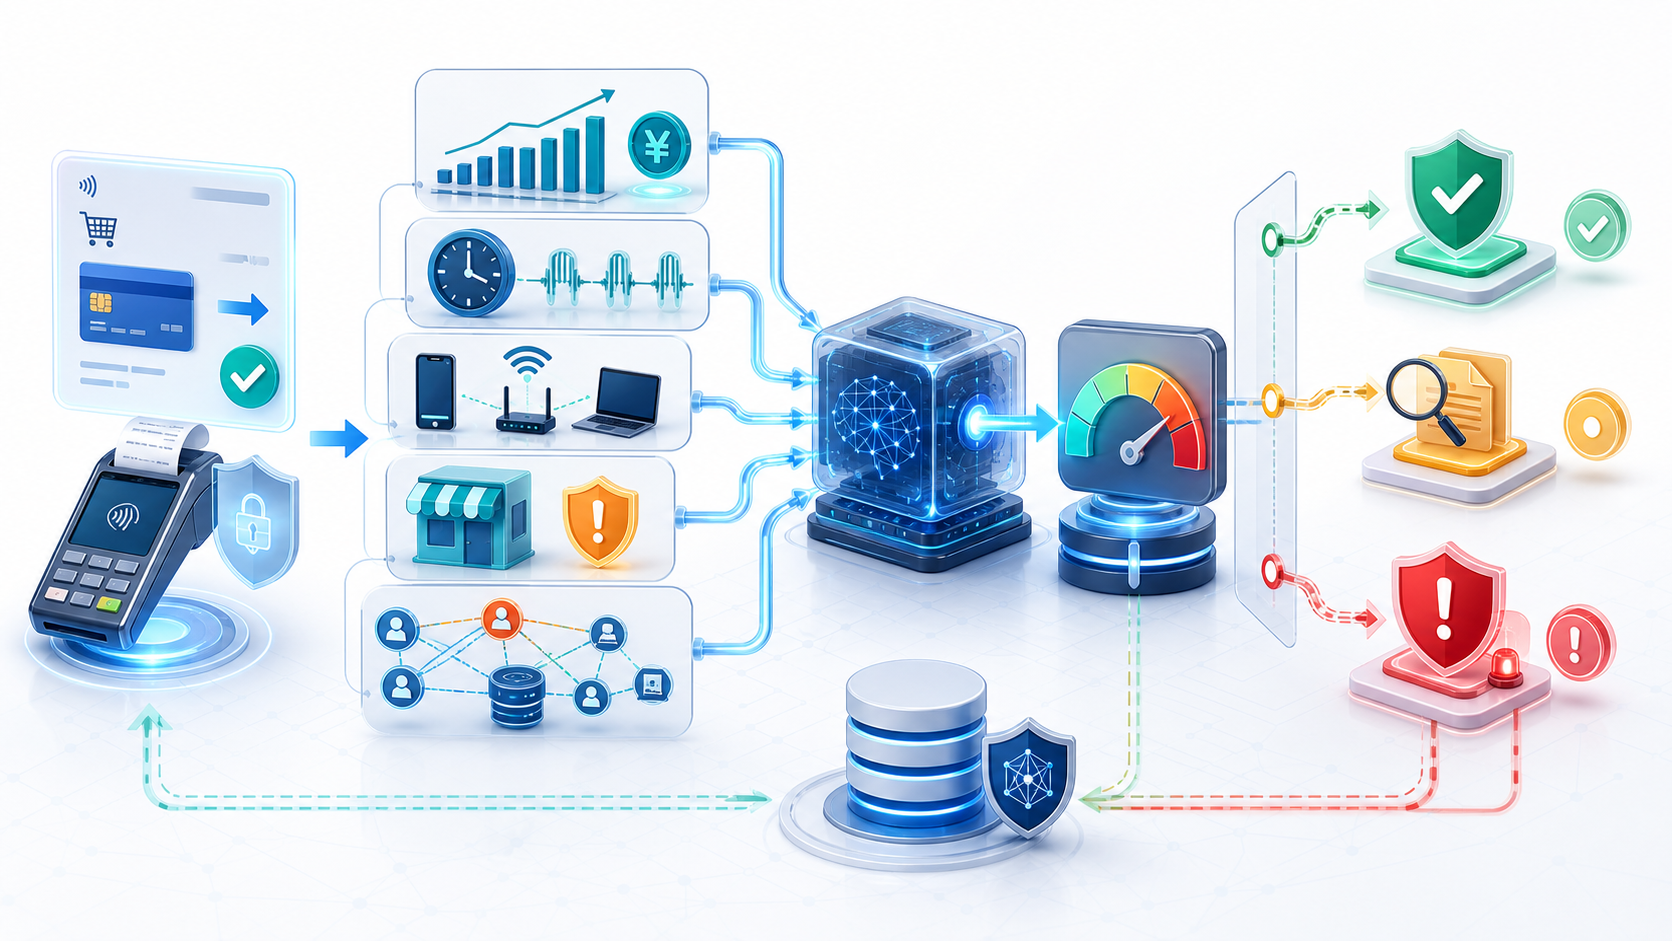
\includegraphics[width=0.92\textwidth]{pic/fraud_analyst_review.png}
  \caption{多维证据融合与诈骗分级判定示意}
  \label{fig:fraud_judgment_illustration}
\end{figure}

Dashboard将风险分数、处置结论、图链路和理由码组织在同一研判界面中，如图~\ref{fig:dashboard_reason_codes}所示。评审人员能够从高风险结论继续下钻到短时高频、共享设备、商户集中和欺诈邻域等具体证据，验证判定结果并非只有黑盒分数。

\begin{figure}[H]
  \centering
  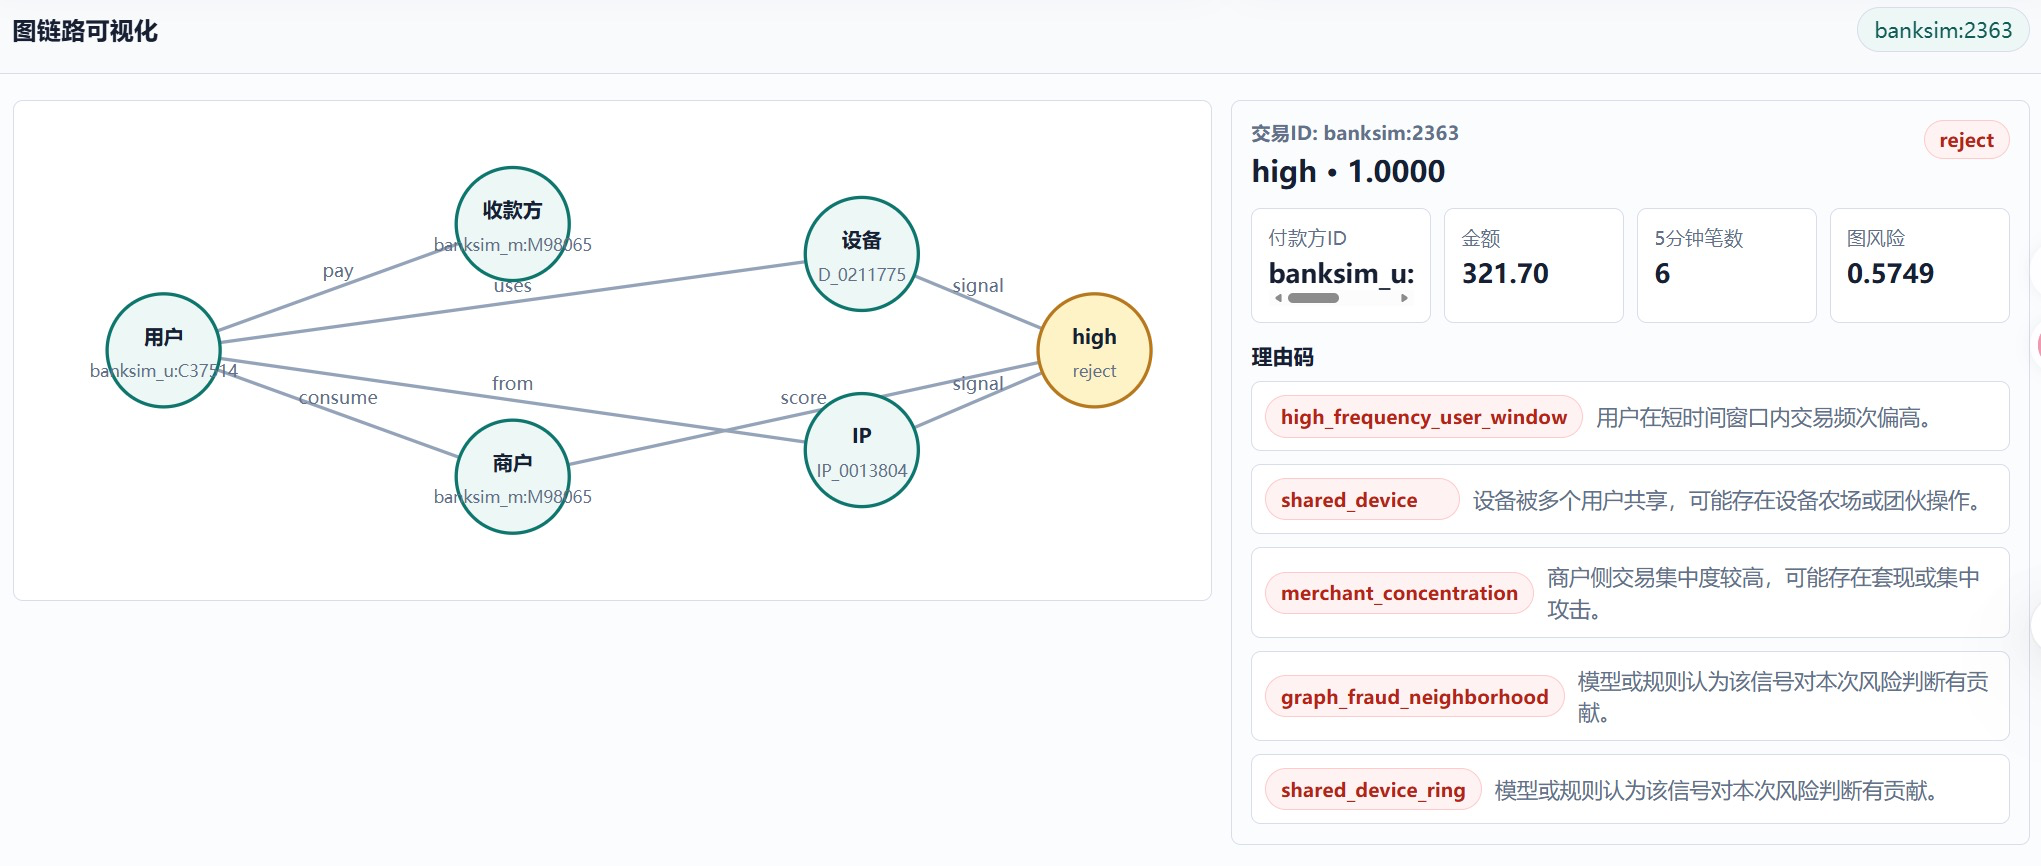
\includegraphics[width=0.96\textwidth]{pic/dashboard_reason_codes_report.png}
  \caption{单笔高风险交易的图链路与理由码解释界面}
  \label{fig:dashboard_reason_codes}
\end{figure}

\subsubsection{诈骗行为建模、图挖掘与团伙溯源}

图挖掘模块以交易、账户、设备、IP、商户和收款方为节点，以交易、登录、设备使用、商户支付、转账等关系为边。模块通过共享资源筛选候选风险资源，再使用并查集构建连通分量，综合欺诈种子比例、用户规模、证据数量、共享设备/IP数量和场景数量计算团伙风险分。

图挖掘输出四类产物：\code{fraud\_groups.parquet}记录疑似团伙列表；\code{entity\_graph\_risk.parquet}记录实体级团伙风险特征；\code{group\_evidence.jsonl}记录共享设备、IP、商户、收款方等证据；\code{graph\_mining\_summary.json}记录挖掘摘要。API提供团伙列表、团伙详情、实体风险和实体关联链路接口，Dashboard支持拖拽和缩放证据图，满足赛题对“可解释性与溯源分析”的要求。

\begin{figure}[H]
  \centering
  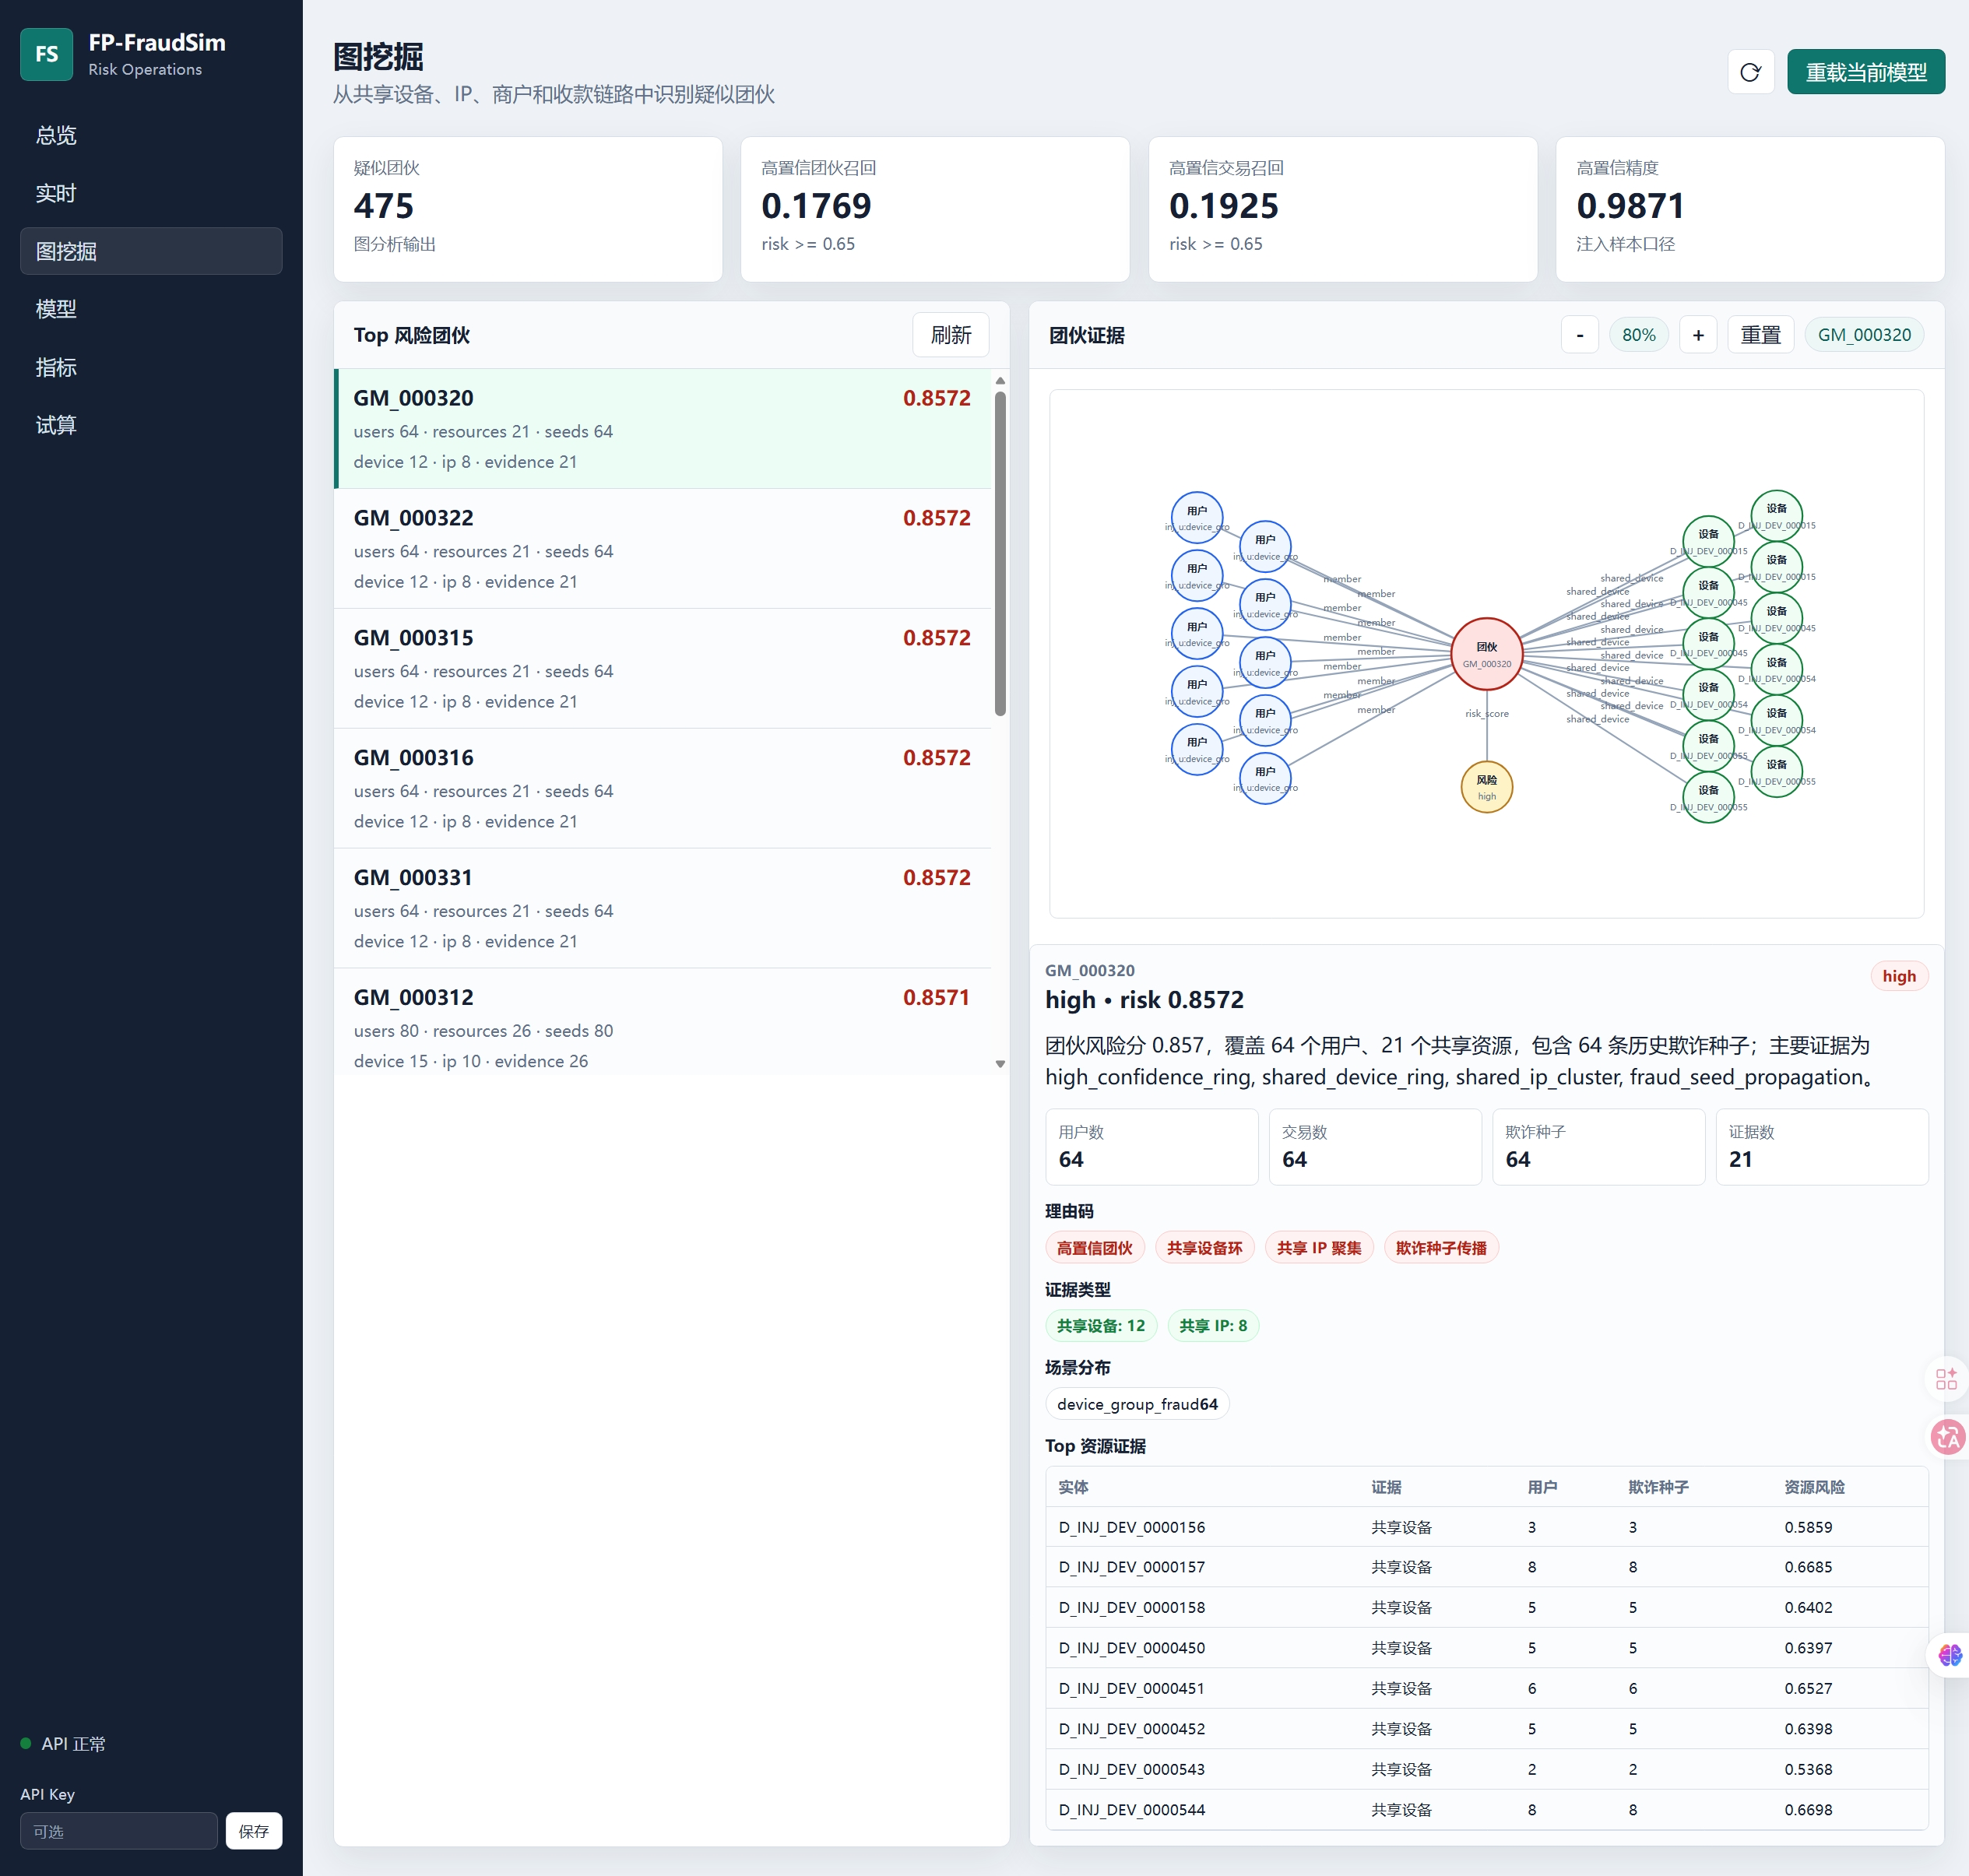
\includegraphics[width=0.76\textwidth]{pic/dashboard_fraud_groups_report.png}
  \caption{疑似欺诈团伙列表、共享资源证据与关系网络界面}
  \label{fig:dashboard_fraud_groups}
\end{figure}

GraphSAGE旁路模块从统一图边中受控采样，使用节点类型、度数和邻居聚合训练两层模型，输出模型、节点嵌入、风险分数和实验指标。线上主模型继续使用稳定的基础图统计，GraphSAGE结果用于创新验证和后续融合研究。

\subsubsection{可视化应用扩展}

Dashboard由Model API静态托管，路径为\code{/dashboard}。页面支持查看健康状态、模型指标、Kafka近期消息、实时告警、单笔试算、人工反馈、模型切换、图挖掘结果、GraphSAGE旁路指标和阈值沙盒。演示按钮封装可调仿真、画像初始化、交易回放、候选重训和图挖掘任务，API返回任务状态与日志尾部，便于在一个界面完成闭环演示。

图~\ref{fig:dashboard_overview}展示了系统总览与核心任务入口，图~\ref{fig:dashboard_replay_feedback}展示了交易回放、实时风险结果、图链路和人工反馈的联动过程。两类界面共同证明系统能够从模型加载状态进入实时识别，并将复核结论重新写回反馈主题。

\begin{figure}[H]
  \centering
  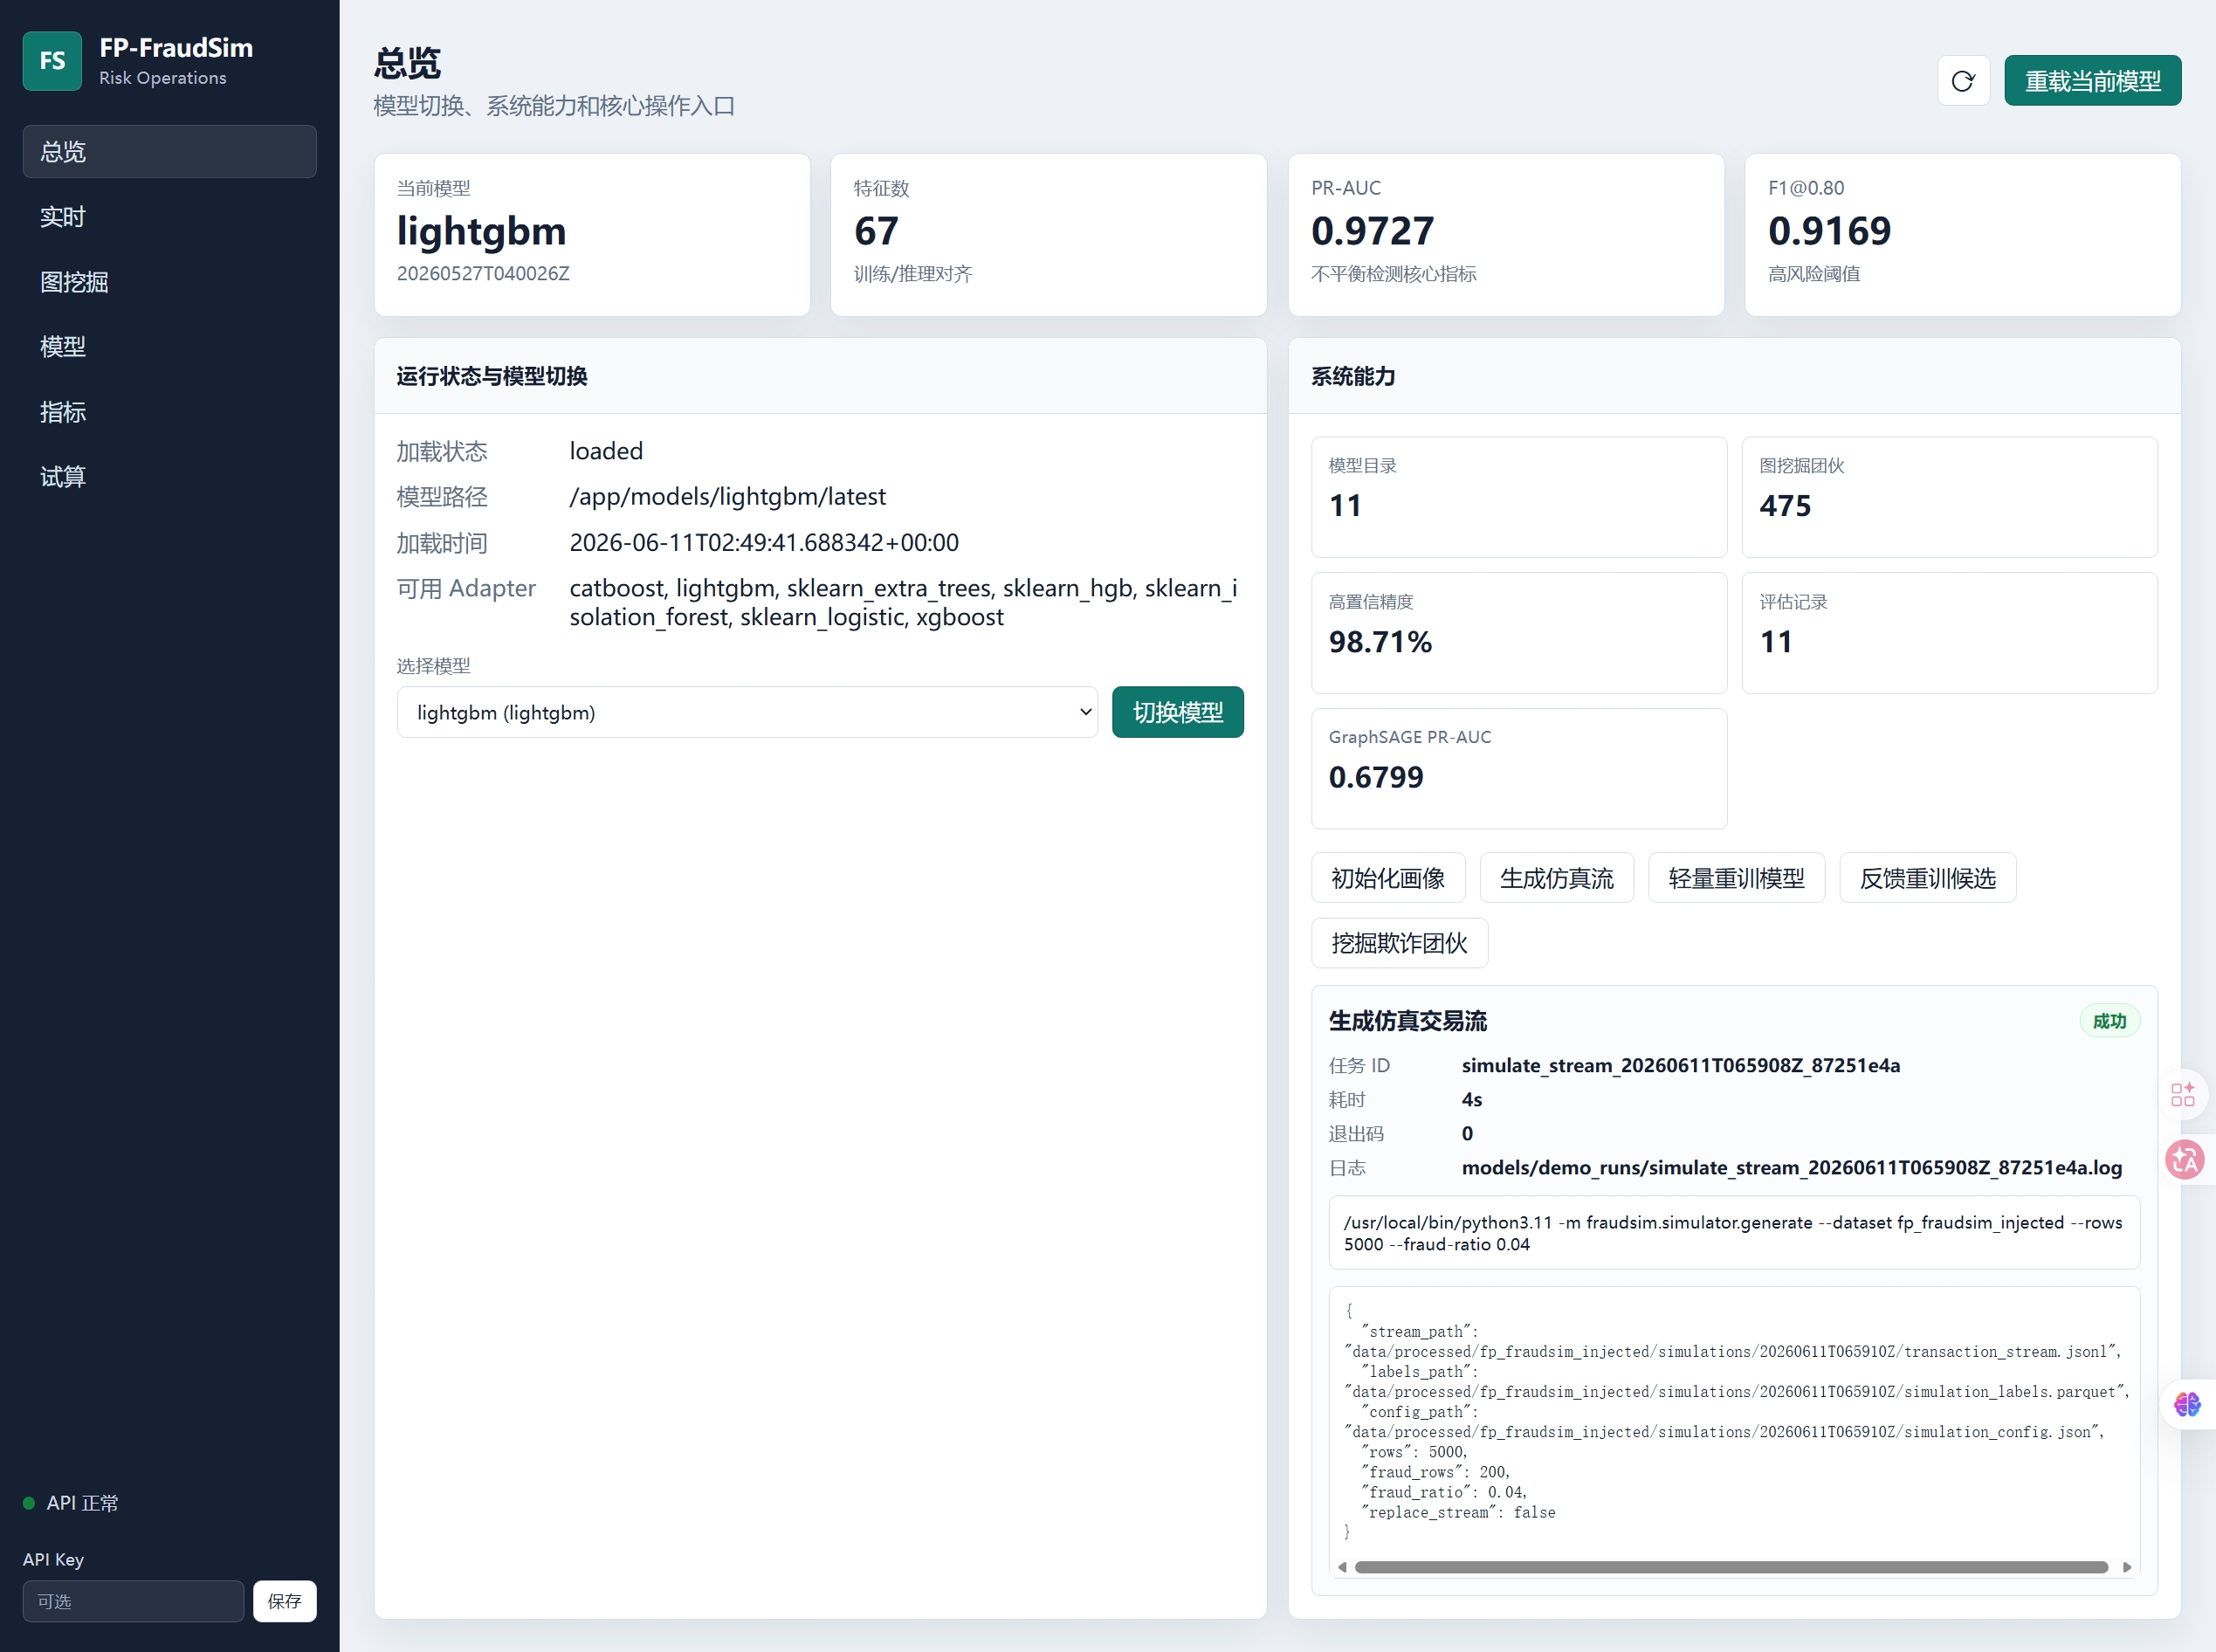
\includegraphics[width=0.90\textwidth]{pic/dashboard_overview_report.png}
  \caption{FP-FraudSim Dashboard总览与核心任务入口}
  \label{fig:dashboard_overview}
\end{figure}

\begin{figure}[H]
  \centering
  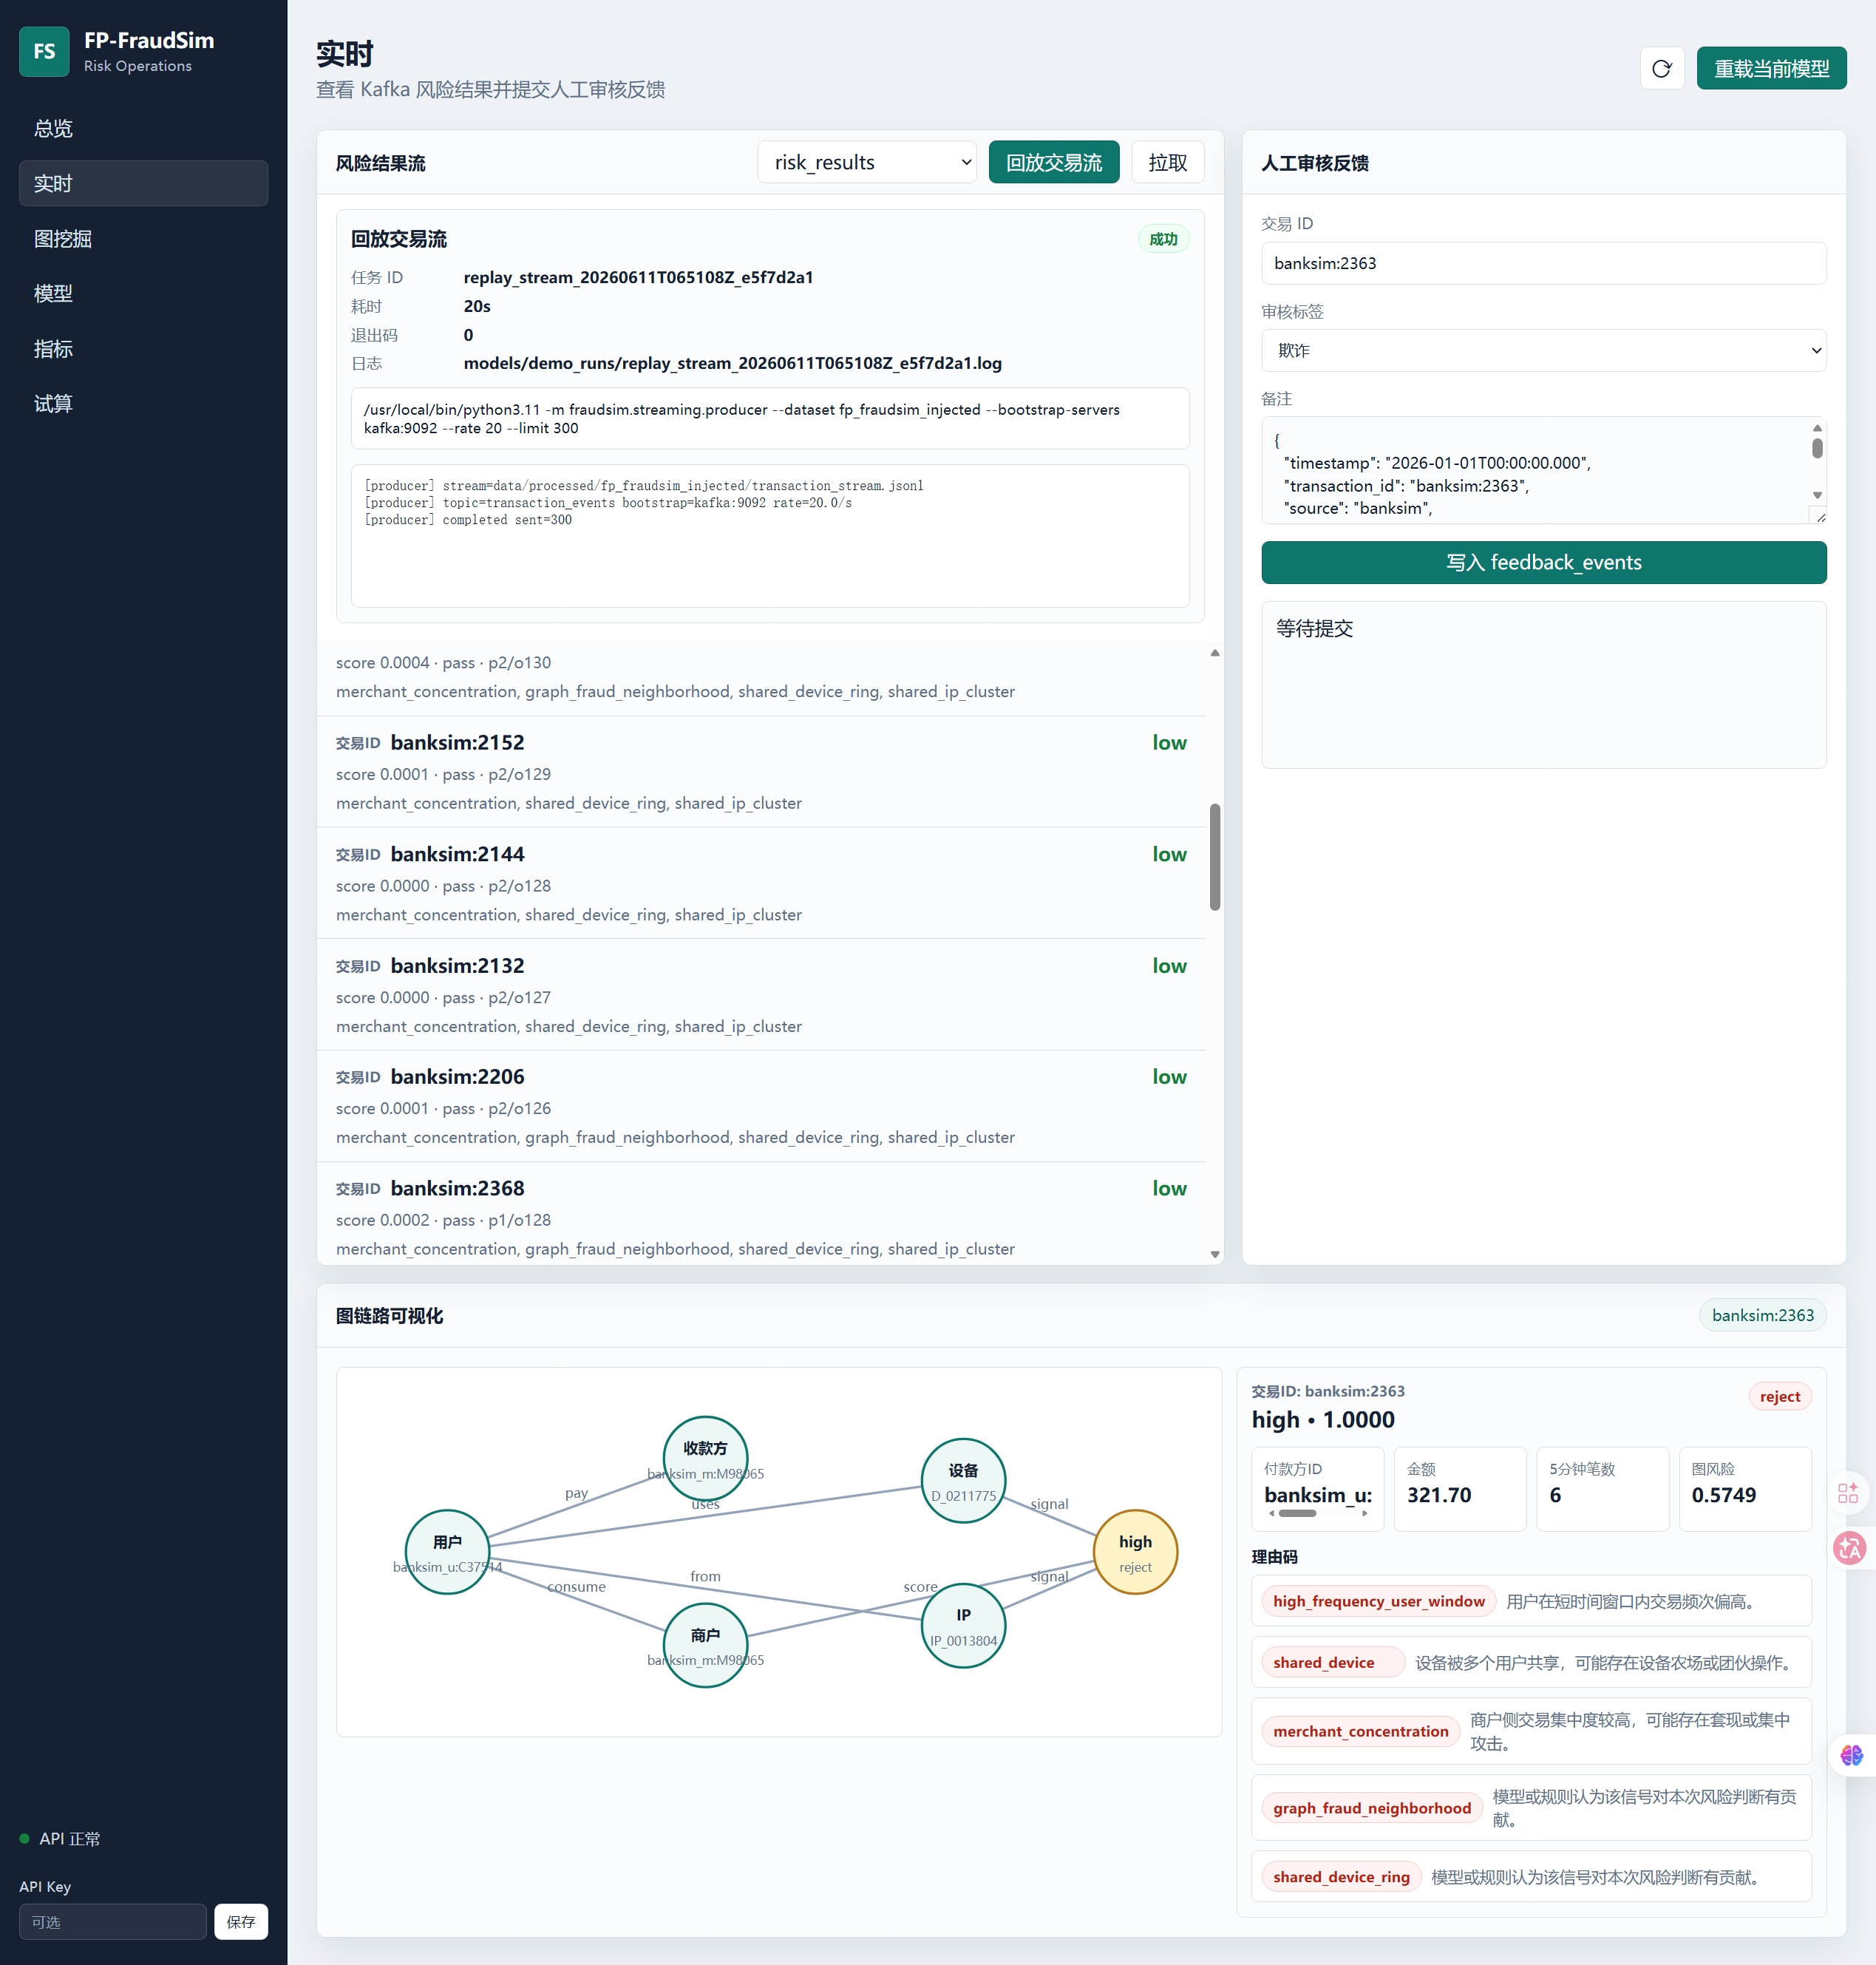
\includegraphics[width=0.74\textwidth]{pic/dashboard_replay_feedback_report.png}
  \caption{交易流回放、实时判定与人工反馈联动界面}
  \label{fig:dashboard_replay_feedback}
\end{figure}
